\documentclass{scrartcl}
% \usepackage{german} % including this twice is causing build fails !!
\usepackage[utf8]{inputenc}
\usepackage[german]{babel}
\usepackage{amssymb} % what does it do?
\usepackage{graphicx} % I can't do that yet
\usepackage{fancyhdr} % what does it do?
\usepackage{lastpage} % what does it do?
\usepackage{multicol} % multicols
\usepackage{advdate}  % advancing day by one (or more)


\AdvanceDate

\setlength{\parskip}{\medskipamount} % thats reasonable
\setlength{\parindent}{0pt} % whatever that does


%%%%%%%%%%%%%%%%%%%%%%%%
% Kopf- und Fusszeilen %
%%%%%%%%%%%%%%%%%%%%%%%%
\pagestyle{fancy}
\lhead{
    \begin{tabular}{ll}
        Felix Karg \\
    \end{tabular}
}
\chead{Bioinformatics Summary}
\rhead{
    \begin{tabular}{rr}
        \today{} \\
        Page \thepage{} of \pageref{LastPage}
    \end{tabular}
}
\lfoot{}
\cfoot{}
\rfoot{}

%%%%%%%%%%%%%%%%%%%%%%%%
% Anfang des Dokuments %
%%%%%%%%%%%%%%%%%%%%%%%%
\begin{document}

\section*{A Simple Protocol for the Inference of RNA Global Pairwise Alignments}


\section*{Recap}

Similiar secondary structures are usually similiar in functionality.


\subsection*{SPS}
Is called the Sum of Pairs Score, Similiarity is: \\
1 - (edit distance / unaligned length of shorter sequence)

\subsection*{Sequence Identity}
The identity is the number of identical nucleotides divided by the shorter sequence length, so a measure for how many parts of the sequences are 'equal' or so to say.


\subsection*{needle}

\verb!needle! is an implementation of the sequence based Needleman-Wunsch
algorithm, which is basically only the classical edit-distance
(Levenstein-distance) algorithm.

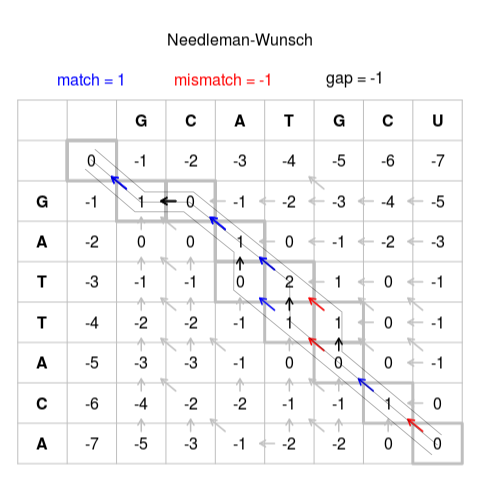
\includegraphics[width=0.6\textwidth]{bioinfI/images/Needleman-Wunsch_pairwise_sequence_alignment}

\newpage

\section*{Tree-based Sequence Alignments}

\begin{itemize}
\item gardenia
\item RNA StrAT
\item RNAdistance
\item RNAforester
\end{itemize}

These are also extensively using the secondary structure for comparison, which
is why they improve a lot with better curated secondary structures.

They are basically doing an edit-distance alignment with a metric that's also
including the secondary structures and it's differences.

As edit operations on trees are basically edit operations on arc-annotated
sequences, this is sometimes used to visualise it instead of some kind of
trees.


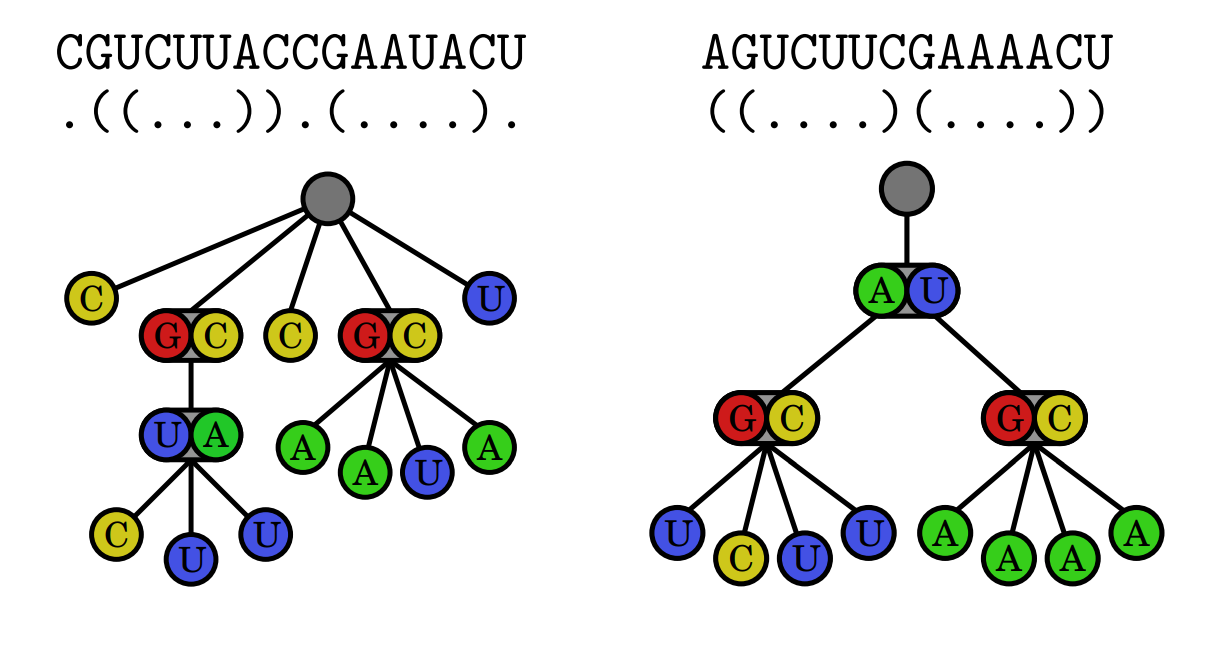
\includegraphics[width=0.7\textwidth]{bioinfII/images/tree_sequences}

Now there's more options for Edit-Distances, having the following
possibilities:
\begin{multicols}{2}
\begin{itemize}
    \item base match
    \item base indel
    \item arc match
    \item arc mismatch
    \item arc breaking (missing arc)
    \item arc altering
    \item arc removing
\end{itemize}
\end{multicols}


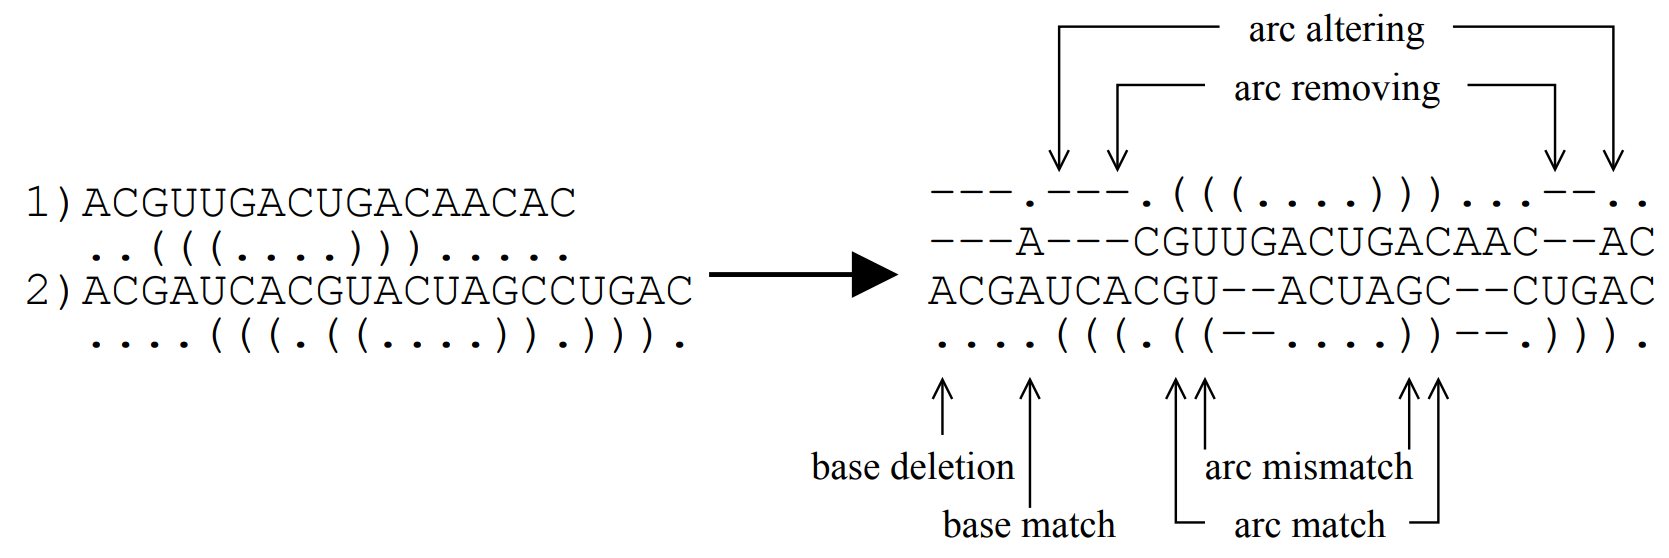
\includegraphics[width=\textwidth]{bioinfII/images/arc_things}



% \subsection*{Sequence Alignment}
% 
% There's three categories:
% \begin{itemize}
% \item local
% \item global
% \item glocal
% \end{itemize}
% 
% Local is comparing (local) parts which are pretty similiar to begin with.
% 
% Global is just comparing two RNA strands, complete.
% 
% Glocal is roughly everything else, having restrictions (beginning/end) when aligning.


\section*{LocARNA}

Is a folding and aligning sequence algorithm. 
First a base pair probability matrix is being created using RNAfold, this is
then used to prune possible arcs. Only these with realistic chances are further
considered.


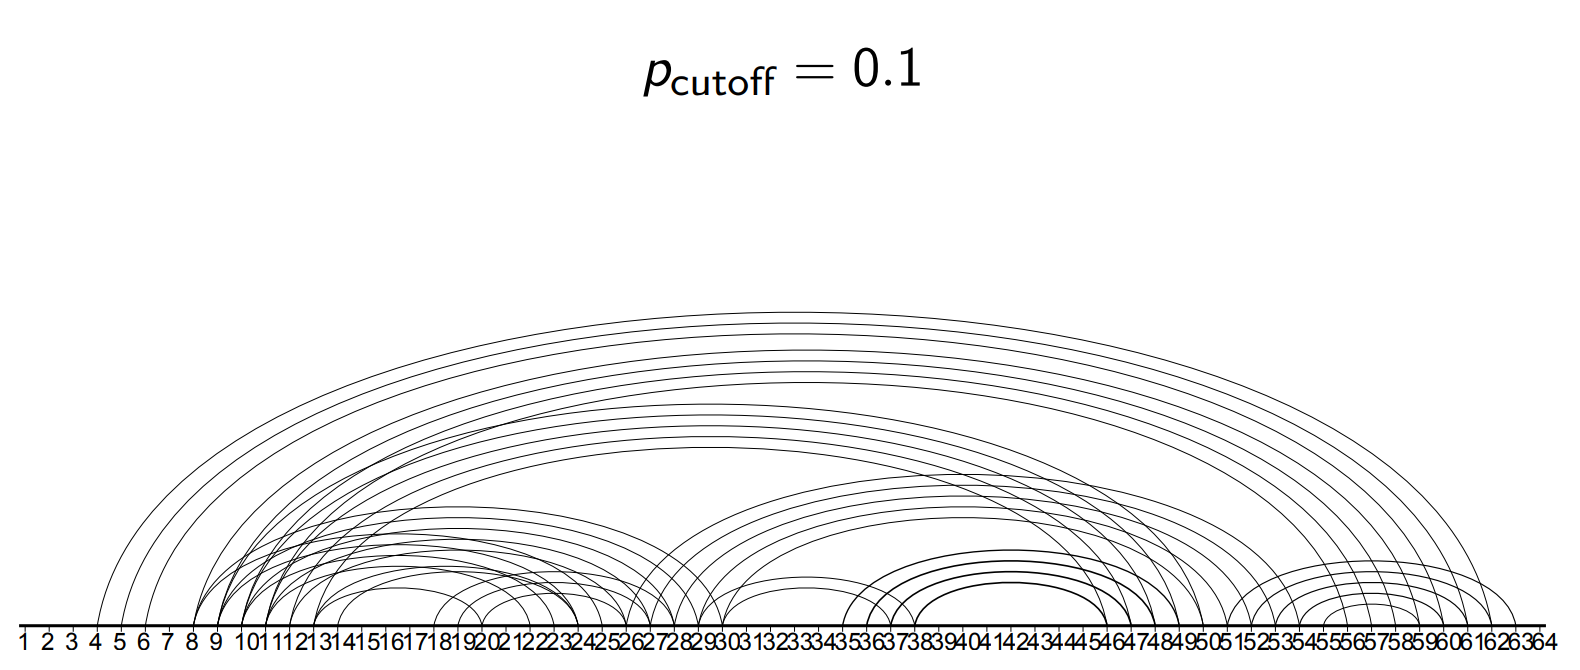
\includegraphics[width=\textwidth]{bioinfII/images/cutoff_01}
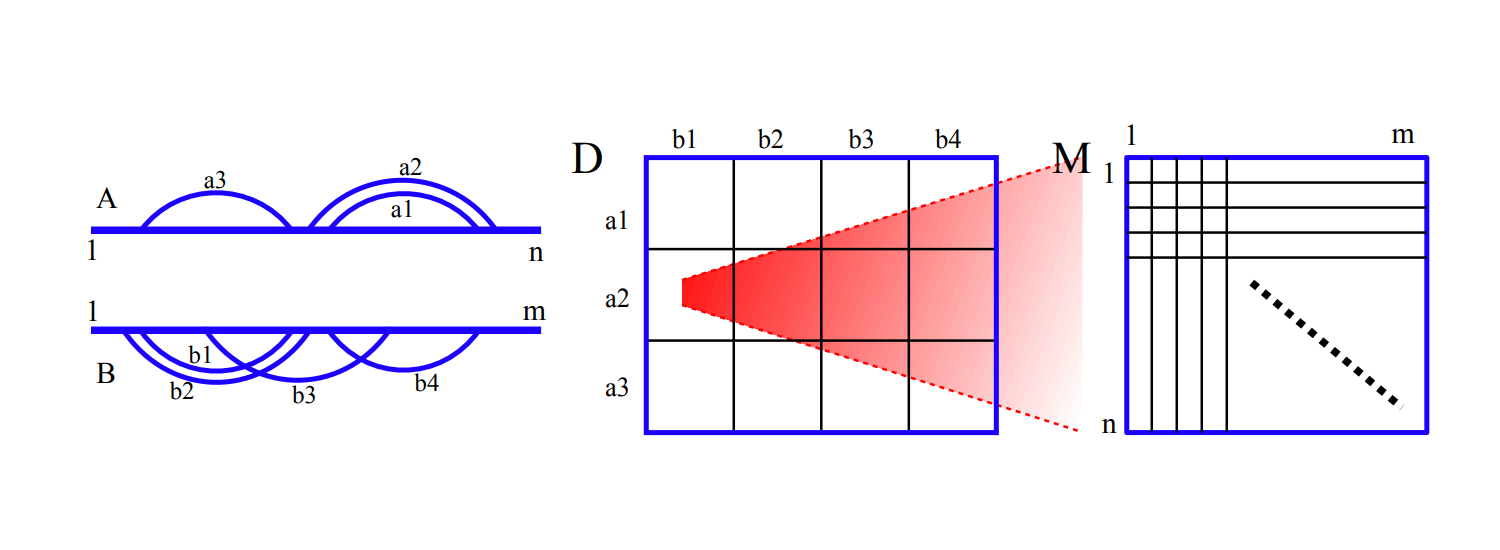
\includegraphics[width=\textwidth]{bioinfII/images/locarnamatrices2}

Then, Alignment scores for all of these realistic arcs are
computed, caching smaller one's first. Meanwhile, the full path matrix is being
filled out with values.



\includegraphics[width=0.3\textwidth]{bioinfII/images/Arcs_example}

\newpage

\subsection*{Comparison}

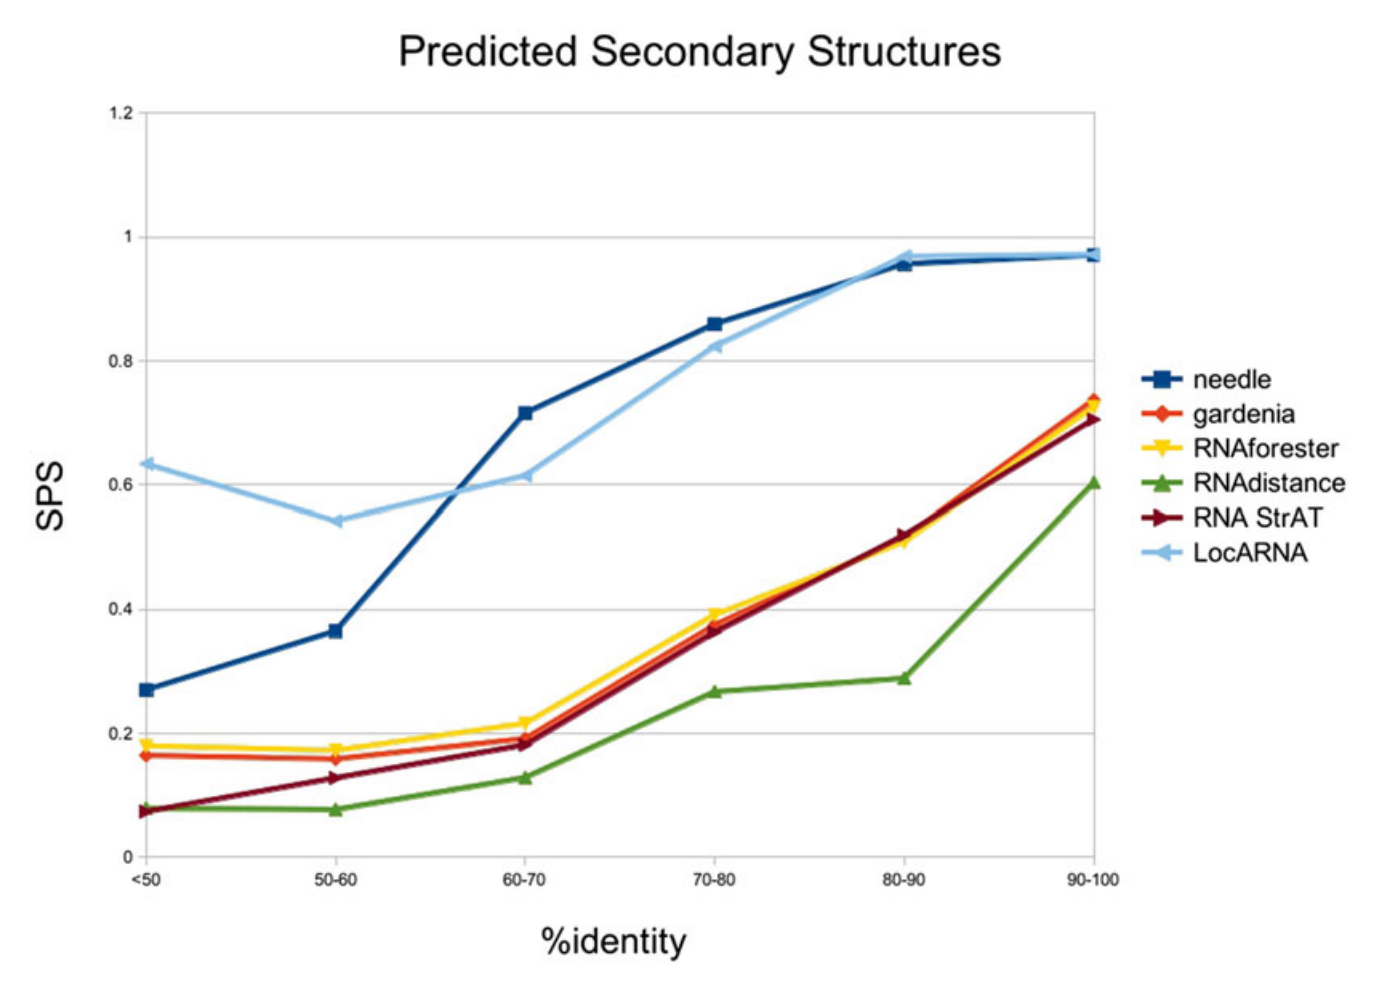
\includegraphics[width=0.53\textwidth]{bioinfI/images/predicted} \\
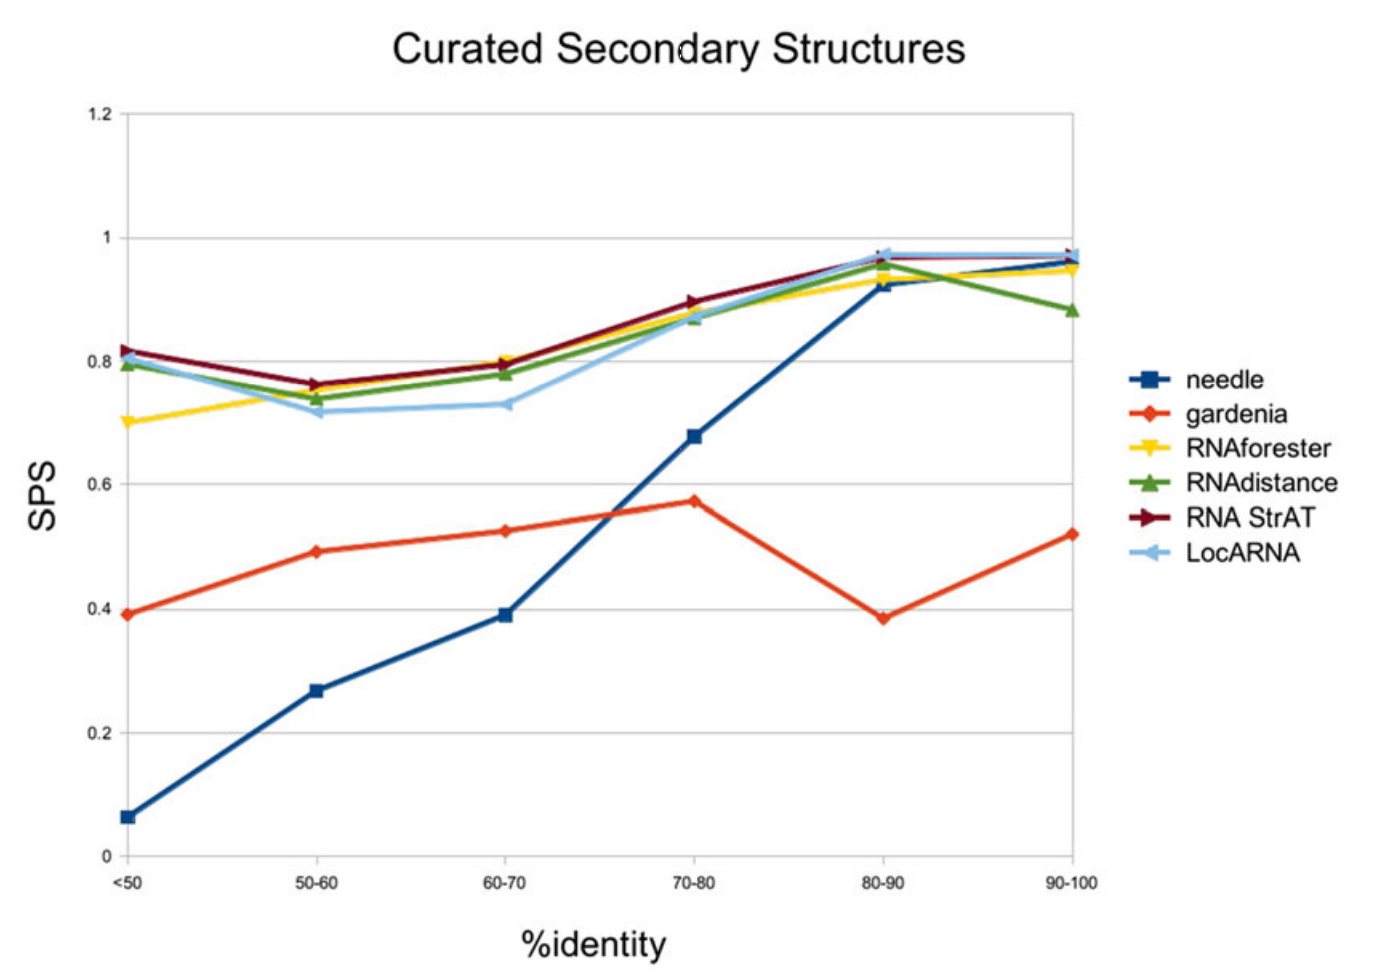
\includegraphics[width=0.53\textwidth]{bioinfI/images/curated} \\
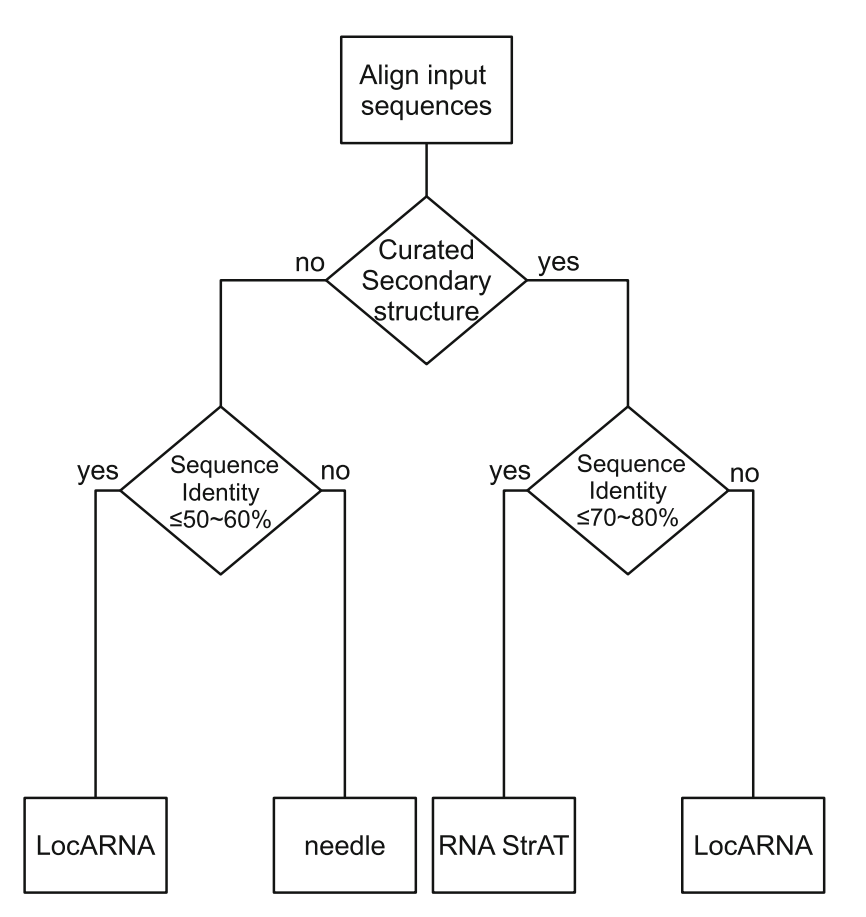
\includegraphics[width=0.53\textwidth]{bioinfI/images/flow}


\verb!https://github.com/fkarg/things-to-talk-about/tree/master/bioinfII!

\end{document}


